\chapter{Lezione 2 - Enterprise resource planning}

Benvenuti a tutti a questa lezione sull'enterprise resource planning, gestione delle risorse di un'impresa, di un'azienda o di un'organizzazione.
Quali sono gli argomenti che affronteremo in questa lezione?

Argomenti trattati:

\FloatBarrier
\begin{figure}[H]
  \centering
  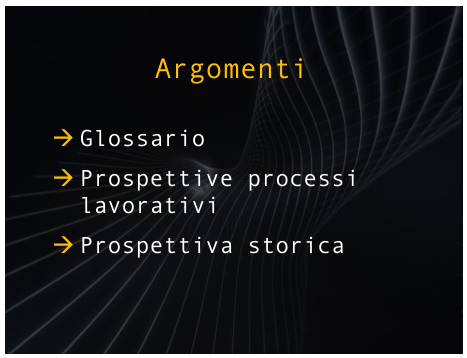
\includegraphics[width=0.50\textwidth,
                    trim=40 80 40 40, % L B R T
                    clip]
                    {images/Lez02_p01_fig_02}
  \caption{Sommario}
  \label{fig:Lez15_p06_fig_02}
\end{figure}
\FloatBarrier
\noindent

Innanzitutto faremo il punto sulla terminologia, quindi vedremo alcune definizioni dei termini, confronteremo alcuni termini più complessi delle locuzioni riguardanti questo settore.
In seguito vedremo quali sono le prospettive da cui vengono analizzati i processi aziendali, sono due prospettive che vedremo.
Da ultimo il terzo argomento che vedremo in questa parte della lezione, faremo una prospettiva storica dei sistemi che sostengono, aiutano nella gestione e nella pianificazione delle risorse aziendali.

\section{Glossario}

Cominciamo col glossario.

\FloatBarrier
\begin{figure}[H]
  \centering
  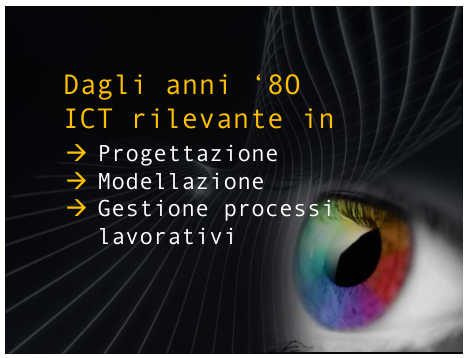
\includegraphics[width=0.50\textwidth,
                    trim=40 80 40 40, % L B R T
                    clip]
                    {images/Lez02_p01_fig_04}
  \caption{Sommario}
%   \label{fig:Lez15_p06_fig_02}
\end{figure}
\FloatBarrier
\noindent

Infatti, dagli anni 80 le tecnologie dell'informazione, della comunicazione e della partecipazione sono rilevanti, sono molto utilizzate nella progettazione ma anche nella modellazione e nella gestione dei processi lavorativi.

\FloatBarrier
\begin{figure}[H]
  \centering
  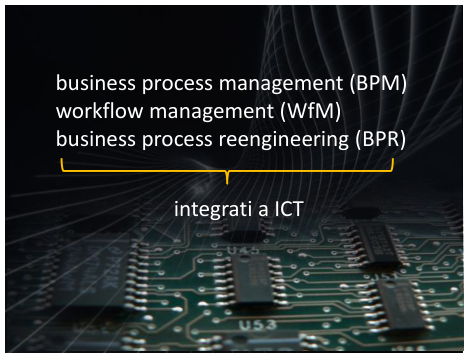
\includegraphics[width=0.50\textwidth,
                    trim=40 130 40 40, % L B R T
                    clip]
                    {images/Lez02_p01_fig_05}
%   \caption{Sommario}
%   \label{fig:Lez15_p06_fig_02}
\end{figure}
\FloatBarrier
\noindent

Nonostante questo, la terminologia business process management, quindi la gestione dei processi organizzativi, la gestione dei processi lavorativi più strettamente e la ringenerizzazione, quindi la rimplementazione e la riorganizzazione dei processi lavorativi, pur essendo integrati con le tecnologie, non hanno trovato una loro specifica collocazione, definizione e caratterizzazione.
Non vi è in altri termini una omogeneità, una chiarezza linguistica.

\FloatBarrier
\begin{figure}[H]
  \centering
  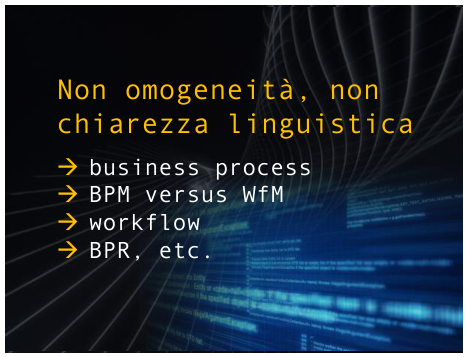
\includegraphics[width=0.50\textwidth,
                    trim=40 80 40 40, % L B R T
                    clip]
                    {images/Lez02_p01_fig_06}
%   \caption{Sommario}
%   \label{fig:Lez15_p06_fig_02}
\end{figure}
\FloatBarrier
\noindent
Business process, per esempio, ha diverse definizioni accettabili parzialmente sovrapposte di questo concetto.
Di conseguenza, la gestione dei processi aziendali non viene caratterizzata immediatamente rispetto all'attività che viene chiamata workflow management, quindi i processi lavorativi più operativi che sono gestiti adesso, come vedremo, automaticamente, fin dalla loro definizione.
Infine, il concetto di workflow e il concetto, la definizione di business process re-engineering e altri connessi.

\subsection{Business process}

Ma vediamo la prima definizione riguardante business process, processi aziendali, processi organizzativi o, in senso più operativo, i processi di lavoro.

\FloatBarrier
\begin{figure}[H]
  \centering
  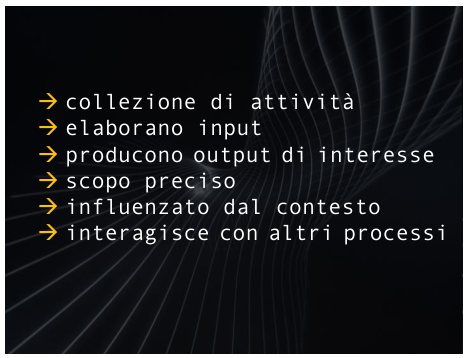
\includegraphics[width=0.50\textwidth,
                    trim=20 80 10 40, % L B R T
                    clip]
                    {images/Lez02_p02_fig_02}
%   \caption{Sommario}
%   \label{fig:Lez15_p06_fig_02}
\end{figure}
\FloatBarrier
\noindent

La prima definizione vede un business process come una collezione di attività che elaborano delle entrate, degli input generici, possono essere informazioni o naturalmente in un processo manifatturiero materiali, sostanze, può essere un'energia in entrata.
Producono un output di interesse, quindi il processo lavorativo deve avere un risultato, ha uno scopo preciso, quindi è un'attività prevista per raggiungere un certo risultato o svolta per raggiungere determinati obiettivi per un certo motivo ed è influenzata dal contesto.
Quale contesto?
Il contesto lavorativo, quindi il contesto di chi svolge questa attività, ma anche il contesto ambientale, il contesto organizzativo.
Questo processo interagisce con altri processi, altri processi della stessa organizzazione o altri processi che sono svolti nell'ambiente.

\FloatBarrier
\begin{figure}[H]
  \centering
  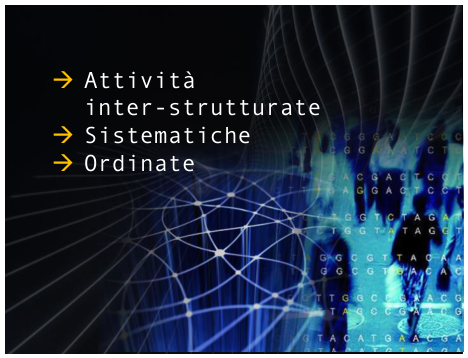
\includegraphics[width=0.50\textwidth,
                    trim=20 80 10 40, % L B R T
                    clip]
                    {images/Lez02_p02_fig_03}
%   \caption{Sommario}
%   \label{fig:Lez15_p06_fig_02}
\end{figure}
\FloatBarrier
\noindent

Ma abbiamo visto che l'inizio della definizione di business process, questa definizione, considera il business process come una collezione di attività, ma noi vogliamo focalizzare questa definizione ad attività strutturate tra di loro, collegate in maniera sistematica e ordinate.

\FloatBarrier
\begin{figure}[H]
  \centering
  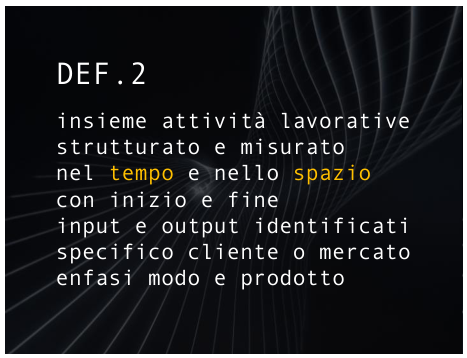
\includegraphics[width=0.50\textwidth,
                    trim=20 40 10 40, % L B R T
                    clip]
                    {images/Lez02_p02_fig_04}
%   \caption{Sommario}
%   \label{fig:Lez15_p06_fig_02}
\end{figure}
\FloatBarrier
\noindent

Quindi la seconda definizione di business process lo considera un insieme di attività lavorative, l'insieme strutturato e misurato nel tempo e nello spazio, che ha un inizio e una fine di svolgimento, elabora dei dati, produce un output identificato che è specifico per un cliente o per un mercato e viene posta enfasi sul modo in cui viene svolto e sul prodotto.
Focalizziamo che il tempo e lo spazio vengono enfatizzati oltre alla strutturazione di questo processo.
Il processo quindi non è disorganizzato, non è casuale, non è anarchico, ed è svolto in un tempo definito e in uno spazio, nel tempo sia per la consequenzialità delle operazioni che abbiamo visto in questa definizione devono essere organizzate, ma anche in un tempo finito.
Naturalmente il processo deve avere un tempo, deve avere una scadenza presumibilmente prevista.
Lo spazio invece perché le attività sono svolte sì nell'ambito dell'organizzazione, ma siamo già nella prospettiva di organizzazioni virtuali e comunque anche in una organizzazione reale le attività possono essere svolte da comunità virtuali.
Quindi la locazione degli attori che svolgeranno questa attività e delle attività stesse non è prevedibile, non è prevista e comunque non è necessariamente inclusa geograficamente nella organizzazione, nella struttura fisica dell'organizzazione.
Ho citato di sfuggita adesso anche gli attori.
Gli attori che svolgono le attività di un processo lavorativo sono gli elementi che caratterizzano la terza definizione che nasce infatti con un focus, l'attenzione sugli attori e la loro collaborazione, la loro interrelazione.

\subsubsection*{Focus su attori e collaborazione}

\FloatBarrier
\begin{figure}[H]
  \centering
  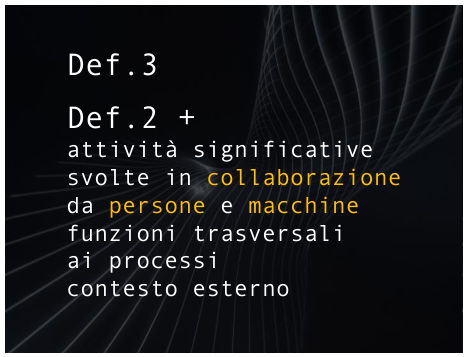
\includegraphics[width=0.50\textwidth,
                    trim=20 80 10 40, % L B R T
                    clip]
                    {images/Lez02_p02_fig_06}
%   \caption{Sommario}
%   \label{fig:Lez15_p06_fig_02}
\end{figure}
\FloatBarrier
\noindent

Quindi la definizione 3 diventa un'estensione della definizione 2 considerando che le attività sono significative svolte in collaborazione da persone e macchine per svolgere funzioni eventualmente trasversali ai processi in un contesto anche esterno.
E' importante qui questa modifica.
Questa è una modifica che considera l'ambito tecnologico collaborativo.
Dove emerge questa idea?
Dove emerge questa interpretazione?
Emerge proprio dalla considerazione che gli attori che svolgono le attività di un processo organizzativo possono essere sia attori umani sia le persone ma anche i device, le infrastrutture tecnologiche che vengono acquisite.
Saranno lavori passivi, saranno lavori coordinati dall'uomo ma intervengono attivamente.
Inoltre si parla di collaborazione.
Un processo lavorativo che abbia un minimo di complessità ecco che deve considerare le interazioni, deve considerare di essere svolto da un gruppo di attori e deve essere svolto da questi attori che interagiscono, in interattività, che collaborano allo svolgimento della stessa attività.
Possiamo a questo punto considerare l'ultima definizione che è una sintesi delle tre definizioni precedente.

\FloatBarrier
\begin{figure}[H]
  \centering
  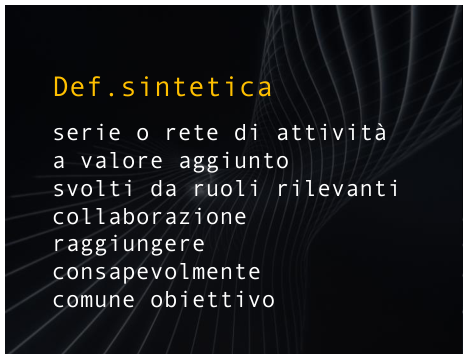
\includegraphics[width=0.50\textwidth,
                    trim=20 40 10 40, % L B R T
                    clip]
                    {images/Lez02_p03_fig_01}
%   \caption{Sommario}
%   \label{fig:Lez15_p06_fig_02}
\end{figure}
\FloatBarrier
\noindent

Quindi il processo lavorativo è una serie o una rete, quindi facciamo riferimento a una struttura di attività a valore aggiunto, quindi devono essere rilevanti, svolti da ruoli quindi da persone o macchine, strumenti tecnologici, rilevanti, in collaborazione per raggiungere consapevolmente un comune obiettivo.
Consapevolmente perché  almeno per gli attori umani la consapevolezza del lavoro che si sta svolgendo e la motivazione sono rilevanti per l'efficacia e l'efficienza della attività.
Ma vediamo ora alcune definizioni riguardanti le attività di gestione di un business process.
Vediamo come è composto il ciclo di vita dell'attività che viene chiamata business process management.

\FloatBarrier
\begin{figure}[H]
  \centering
  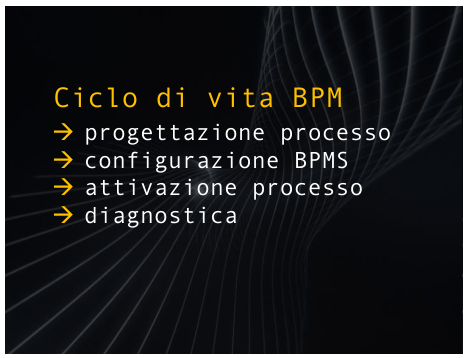
\includegraphics[width=0.50\textwidth,
                    trim=20 100 10 60, % L B R T
                    clip]
                    {images/Lez02_p03_fig_02}
%   \caption{Sommario}
%   \label{fig:Lez15_p06_fig_02}
\end{figure}
\FloatBarrier
\noindent

La progettazione del processo.
La progettazione è già vista come progettazione automatica.
Il processo viene definito in una maniera elaborabile o supportata da una macchina, quindi siamo già nell'ambito tecnologico.
Il business process management è un settore disciplinare, non una tecnologia, ma fa riferimento a concetti dell'ambito informatico.

La seconda fase del ciclo di vita è la configurazione del sistema di supporto al business management.
La configurazione sia dell'ambito lavorativo, quindi la definizione dei ruoli, delle risorse, la precisazione del contesto lavorativo, sia anche la configurazione effettiva del sistema tecnologico di supporto in termini di personalizzazione funzionale, quindi l'aggiunta di eventuali strumenti, ma anche il settaggio, la definizione dei parametri per il suo corretto funzionamento.

L'attivazione del processo.
Il processo definito nella prima fase viene attivato, eseguito dalla macchina, dal calcolatore.
In questo caso vorrei focalizzare, due situazioni.
La situazione del manufacturing, per esempio, della fabbrica automatica in cui il processo può essere eseguito automaticamente, quindi una macchina a controllo automatico, oppure in un altro ambito il computer, il sistema automatico, che sostiene in qualche modo il controllo dell'attività, del corretto svolgimento delle attività, quindi la sequenzialità, la preparazione dei dati e così via.

Infine la diagnostica che serve per il controllo dell'effettivo svolgimento, seppur automatico, del processo, il controllo del corretto avvicinamento alla realizzazione degli obiettivi aziendali e gli eventuali colli di bottiglia che possono inficiare l'efficienza dello svolgimento del workflow e le eventuali rilevate via di fuga, percorsi, situazioni che possono in qualche modo rallentare o creare problemi allo svolgimento automatico del workflow.

\subsubsection*{Businnes Process Reengineering}

\FloatBarrier
\begin{figure}[H]
  \centering
  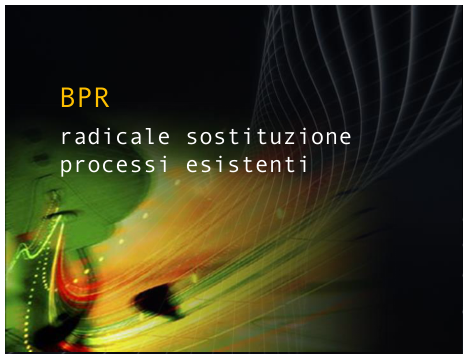
\includegraphics[width=0.50\textwidth,
                    trim=20 160 10 40, % L B R T
                    clip]
                    {images/Lez02_p03_fig_03}
%   \caption{Sommario}
%   \label{fig:Lez15_p06_fig_02}
\end{figure}
\FloatBarrier
\noindent


%14:03 ------------------------------------------------------------------------

Cos'è?
Come viene definito il business process reengineering?
Business process reengineering è un'attività di radicale sostituzione dei processi esistenti.
Diciamo che è in qualche modo un'attività più estrema, più drastica rispetto al cambiamento indotto nell'organizzazione e rispetto al business process management.
Nel business process management vedremo nella definizione precisa i processi vengono riorganizzati sulla base degli esistenti modificati.
Nel reengineering i processi possono essere completamente riprogettati e riempimentati, quindi verso una discontinuità organizzativa della impresa.
Una definizione di business process management viene dalla Gartner.
Gartner è una multinazionale di consulenza tecnologica, ricerca e analisi nell'ambito delle tecnologie, dell'informazione, della comunicazione e della collaborazione fondata nel 1979 e ha proposto questa definizione che è adesso abbastanza Business process management è una disciplina di gestione dei processi.
Abbiamo detto che non è una tecnologia, non richiede, anche se auspica, il supporto, ma non richiede come risultato lo sviluppo di nuovi strumenti, di tecnologie.
Studia i metodi di gestione dei processi.
Quindi non è una tecnologia, ma è sostenuta dalla tecnologia del workflow management.
Inoltre si occupa nella sua attività della raffinazione di processi esistenti.
Raffinazione, quindi, modifica, adattamento, armonizzazione di quanto già esistente nella organizzazione.
È un metodo pratico, iterativo, incrementale.
Vediamo ora una definizione proposta dalla workflow management coalition.
Worldflow management coalition è un consorzio costituito nel maggio del 1993 da alcuni partner commerciali come la Black Forest, l'IBM, la Hewlett Packard, Fujitsu, ICL e 300 tra software e service houses.
È stata definita per la definizione di norme per l'interoperabilità in ambito di workflow management system.
La definizione di norme, non necessariamente la certificazione o il controllo dell'attuazione di queste norme.
La definizione proposta dalla workflow management coalition è la seguente.
Worldflow management si riferisce all'automazione di un processo lavorativo, alla gestione dei documenti prodotti durante lo svolgimento delle attività dai vari attori.
Documenti, informazioni che riguardano l'attività e le attività che vengono scambiati appunto tra gli attori che svolgono le attività.
Ricordo che gli attori possono essere attori umani o possono essere supporti tecnologici.
Ultimo punto, vengono rispettati, devono essere rispettati dei protocolli.
Protocolli per la comunicazione tra i vari attori, protocolli per lo svolgimento corretto dell'attività.
Ogni task può essere eseguito subito dopo aver ricevuto l'input, quindi subito dopo lo svolgimento, la conclusione del processo precedente, e protocolli di interoperabilità.
Vedremo che l'architettura dei sistemi che sostengono la gestione dei workflow sono sistemi integrati.
Sistemi integrati vuol dire che sono utilizzati diversi elementi, diversi applicativi, diversi sistemi realizzati anche indipendentemente.
Quindi è molto importante aver definito a priori dei protocolli standard per l'interoperabilità, quindi per la comunicazione, per lo scambio di significati collettivamente riconosciuti.
Business process management però attualmente è carente di diagnostica.
Business process management è sostenuto dai sistemi di gestione dei workflow, ma viene in qualche modo a sovrapporvizi, proprio per questa carenza di funzionalità nella gestione degli errori della messaggistica.
A questo punto avendo concluso il primo argomento della lezione vorrei proporvi alcuni spunti di riflessione.
Quindi vi propongo di definire un processo lavorativo, un workflow, e confrontare anabitamente questo esempio con la definizione che abbiamo fornito, la definizione della workflow management coalition.
Vediamo ora le prospettive dei processi lavorativi, quindi da che punto di vista vengono analizzate in questo ambito di studio.
Vi sono due prospettive sostanzialmente, vedremo una prospettiva gerarchica, una prospettiva funzionale.
Iniziamo con la prospettiva gerarchica.
La prospettiva gerarchica intuibile dalla locuzione stessa focalizza sull'organigramma, la struttura organizzativa dell'organizzazione, dell'azienda, dell'impresa.
Quindi pone l'accento sulla segnazione dei ruoli e le rispettive responsabilità, i diritti di accesso o di svolgimento delle attività, i livelli di autorità, diciamo, nell'ambito dell'organizzazione.
Definisce quindi una gerarchia dei processi lavorativi, gerarchia che dipende proprio dalla gerarchia definita dall'organigramma.
La gerarchia dei processi gestionali è stata proposta e studiata da Anthony ed è diventato un modello di organizzazione aziendale consolidato per parecchio tempo e tradizionale.
Prevede tre livelli.
Il primo livello riguarda il controllo operativo.
Il controllo operativo assicura l'efficienza e l'efficacia delle attività, raccoglie ed elabora dati dall'attività operative, dall'attività del quotidiano.
Il secondo livello riguarda il controllo gestionale, assicura quindi che le risorse necessarie siano disponibili e utilizzate con efficacia e efficienza in direzione del raggiungimento degli obiettivi previsti dall'organizzazione.
I dati utilizzati a questo livello, i dati elaborati per il decision making a questo livello, riguardano dati più sintetizzati, i dati che riguardano i dipartimenti, i vari settori aziendali.
Siamo ancora all'interno dell'azienda ma aree tematiche o gestionali dell'azienda.
L'ultimo livello è il livello strategico, il livello della pianificazione strategica, in cui vengono definiti gli obiettivi dell'organizzazione o i cambiamenti di obiettivi predefiniti, predecisi, le risorse che servono a dedicare per il raggiungimento di questi obiettivi e le politiche da adottare per ottenere queste risorse.
A questo livello vengono decisi obiettivi considerando anche la concorrenza o gli stakeholders, i fornitori o gli attori del mercato esterni all'organizzazione.
I dati che vengono elaborati, acquisiti ed elaborati a questo livello, riguardano quindi l'intero mercato.
Non sono più dati esclusivamente interni allo svolgimento dell'azienda ma devono essere confrontati le situazioni ambientali e di altre organizzazioni per un confronto.
Vediamo adesso l'altra prospettiva, l'altro punto di vista da cui sono studiati i processi lavorativi, la prospettiva funzionale.
Il focus è quindi sui processi e naturalmente sui ruoli funzionali che li svolgono, quindi sulle competenze interne all'organizzazione.
L'organizzazione dal punto di vista funzionale è vista organizzata in tre classi di attività.
Le core business che sono le attività principali caratterizzanti l'organizzazione, le attività che generano i profitti previsti dall'organizzazione o i profitti in termini economici o in termini di raggiungimento degli obiettivi.
Le attività gestionali, le attività gestionali sono le attività di sostegno, le attività di coordinamento garantiscono l'efficienza e l'adeguatezza dell'impresa e il suo governo, quindi la gestione operativa.
Da ultimo vi sono le attività di supporto, non generano guadagni ma sono comunque rilevanti per gli obiettivi dell'azienda.
Spesso sono attività date in gestione all'esterno, come si dice adesso in outsourcing.
A questo punto, alla fine di quest'argomento, vorrei proporvi uno spunto di riflessione.
Fate un esempio di gerarchia dei processi decisionali in un'organizzazione a scelta.
Vi darei un suggerimento.
Cominciate a individuare un'organizzazione specifica, un'organizzazione che conoscete, che frequentate, che sia un'organizzazione commerciale, un'organizzazione didattica, la vostra organizzazione lavorativa dove lavorate o un'altra.
Definite la, descrivetela e andate a individuare i vari processi decisionali.
Dunque non abbiamo chiesto la gerarchia dell'organigrama, la gerarchia delle funzioni, ma abbiamo chiesto i vari processi con l'ordine gerarchico in cui vengono svolti.
Bene, ora passiamo al successivo argomento che è una prospettiva storica.
Vorrei adesso commentarvi, mostrarvi l'universo dei vari applicativi, sistemi integrati, sistemi complessi, software, classificati relativamente alla loro generalità rispetto all'uso che se ne può fare, e proiettare questa gerarchia nel tempo.
Vediamo.
L'universo dei sistemi software disponibili viene così organizzato in una gerarchia.
Al primo livello, il livello basso, i sistemi operativi sono i programmi che permettono la gestione basilare dei sistemi tecnologici, dei sistemi informatici, quindi l'uso delle risorse di memorizzazione, la gestione del file system, il collegamento in rete, le stampanti e tutti gli altri device.
Al livello successivo troviamo quelli chiamati applicativi generici, sono anche riferiti come software di base, sono applicativi destinati a usi più avanzati delle funzioni primarie offerte dal sistema operativo, ma general purpose, destinate a un ampio spettro di utenti, a un ampio spettro di organizzazione.
A questo livello quindi fanno parte i sistemi per la gestione delle basi di dati, foglie elettronici, i sistemi per la composizione, per l'editing basilare.
A livello successivo troviamo gli applicativi specifici.
Gli applicativi specifici sono rivolti ad attività specifiche dell'azienda o attività di aziende specifiche o di dipartimenti monotematici delle organizzazioni.
A questo livello quindi troveremo sistemi di supporto alle decisioni, software per la gestione, per il sostegno di call center, applicativi specifici per l'editoria elettronica, per la gestione di immagini audio e video ad esempio.
A livello successivo troviamo gli applicativi fatti su misura, sviluppati su misura per soddisfare esigenze specifiche delle organizzazioni dipendenti sia dalla caratterizzazione della specificità della organizzazione sia dalle situazioni o dalle necessità contingenti.
Negli anni 60 esistevano solo i primi due livelli, cioè su un sistema operativo semplice, elementare, venivano sviluppate applicazioni su misura.
Ma questo cosa ha portato?
Questo ha portato allo sviluppo di una miriade di applicativi specifici.
Quindi negli anni 80 l'evoluzione è stata lungo due binari.
Su un binario la ricerca di progettazione di sistemi generali, quindi essendoci resi conto che prosperava lo sviluppo di sistemi specifici, di sistemi sviluppati su misura, si è cominciato a considerare la necessità di disporre di sistemi generali eventualmente specializzabili.
Ci si è resi conto anche di un'altra questione, che molti software potevano essere riutilizzati per lo sviluppo di applicazioni analoghe, cioè dovendo sviluppare applicazioni specifiche il software non era facilmente riutilizzabile, bisognava riscrivere l'intero applicativo.
A questo punto compaiono, sono stati sviluppati gli approcci tipo l'orientamento a oggetti adottato sia nella progettazione sia poi nella programmazione, quindi nello sviluppo di una quantità di linguaggi basati su questo approccio.
Nella fase 2 di assemblaggio dei sistemi complessi basati, assemblaggio basato su riuso di software già sviluppato, partiamo da due livelli di cui uno gli applicativi su misura e il livello degli applicativi specifici si sono estesi, sono cresciuti.
Adesso questi applicativi collaborano a creare, a far nascere il livello degli applicativi generici, applicativi generici che possono poi essere specializzati nei due livelli superiori.
Usciamo adesso dalla visione gerarchica.
Negli anni 70-80 noi abbiamo assistito alla fede in un approccio, al seguito di un approccio data driven.
L'approccio data driven significa che l'organizzazione dei dati, quindi la definizione delle funzioni per il loro processing, per la loro elaborazione, conducevano lo sviluppo, conducevano la guida verso la soluzione dei problemi presentati.
Quindi l'approccio partiva da soluzioni per l'archiviazione, per il recupero o per la modellazione dei dati, strumenti che supportavano questo tipo di attività.
Esistono sistemi di office automation, cominciano a essere sviluppati sistemi di office automation, possiamo ricordare per esempio la nascita della metafora della scrivania piuttosto che applicativi quali office o in seguito open office.
Ma che caratteristica hanno?
Hanno la caratteristica di da una parte riferirsi a un modello specifico di lavoro, stabile di lavoro, dall'altra parte si riferiscono ad attività di back office, quindi attività all'interno della organizzazione.
Non abbiamo ancora rivolto lo sguardo verso da una parte gli altri stakeholder, i possibili partner, i fornitori, i concorrenti, i possibili nuovi partner e dall'altra parte ai customer, ai clienti.
Quindi non c'è ancora la mentalità per lo sviluppo di customer relationship management system.
Inoltre in questi anni ricordo lo sviluppo di internet non è ancora diffuso, sia i servizi sia le connessioni non hanno il livello tecnologico e di potenza attualmente disponibile.
Dobbiamo aspettare infatti gli anni 90 per poter uscire da questa fase di staticità del modello di riferimento.
Questo avviene in seguito nella fase 3, quando viene finalmente adottato l'approccio orientato ai processi, l'enfasi e sulla gestione dei processi.
L'impulso visto negli anni 90 sui sistemi per la gestione dei processi viene da due fattori.
Uno, come abbiamo già detto in precedenza, lo sviluppo delle tecnologie di rete sia la larghezza di banda, sia d'altra parte l'ampiezza, la varietà dei servizi offerti, ma dall'altra parte anche da un problema specifico che doveva essere risolto.
Il passaggio dall'anno 1999 a 2000 è la contemporanea entrata in uso dell'euro, che induceva interventi piuttosto pesanti e diffusi sui sistemi allora esistenti.
Inoltre, nel 90 d'altra parte, pur cominciando lo sviluppo, la diffusione dei sistemi orientati ai processi, dobbiamo però verificare una carenza, la mancanza di standard sia di interoperabilità, sia standard di riferimento per le architetture dei sistemi di process management.
Questa evoluzione viene nella fase 4.
Internet è diffusa, il metodo di sviluppo del software, di progettazione del software basato sul riuso, evolve verso i sistemi modificati al volo, quindi sistemi su cui è possibile intervenire per aggiornamenti, ma d'altra parte ancora più drastico, gli interventi dei sistemi component-based.
Sono sistemi generali, generici, quindi posti al secondo livello che possono essere configurati e stesi specializzati con elementi prodotti per offrire risoluzioni specifiche a problemi.
Quindi applicativi del secondo livello, sistemi del secondo livello che possono essere integrati, sviluppati a diventare del terzo livello.
Quindi i livelli di software terzo e quarto sono visti in qualche modo come un deposito di applicativi per lo sviluppo dei livelli più bassi o meglio dei livelli più generali.
Vediamo ora come i sistemi a cui abbiamo fatto riferimento nel nostro ambito sono collocati.
I sistemi per la gestione del business process del secondo livello attualmente coincidono, come avevamo accennato, ai sistemi per la gestione dei workflow.
Mancano i sistemi di gestione della diagnostica, quindi i sistemi non si differenziano.
Al terzo livello troviamo sistemi per la enterprise resource planning system che contengono come moduli integrati o meglio come componenti integrati sistemi per la gestione dei workflow.
A questo punto l'ultimo argomento della lezione è concluso e passerei a proporvi uno spunto di riflessione.
Provate a concepire un esempio di applicativo o a scegliere tra quelli di vostra conoscenza disponibili un applicativo per ogni fase dell'evoluzione dei sistemi software che abbiamo visto e motivate la collocazione che avete posto.
La lezione è conclusa, ricordo che il materiale didattico per la lezione lo trovate assieme a materiale per eventuali approfondimenti o dettagli sulla sezione opportuna del sito dell'università.
A presto.
La lezione a questo punto è completa, vi ricordo che il materiale didattico per dettagli, approfondimenti, potete trovarlo nell'apposita sezione didattica del sito dell'università.
A presto.
